\section{Lecture 3}

The meaning of the Lorentz Invariant is that \textbf{events}, like $\left( E,F \right)$ exist before I define coordinates. It is a property of the two events.

So to recap what we did in the last lecture, be:
\begin{equation}
x_{E}^{\mu } \text{ and } x_{E}^{\mu'}
\end{equation}
        
\bigskip
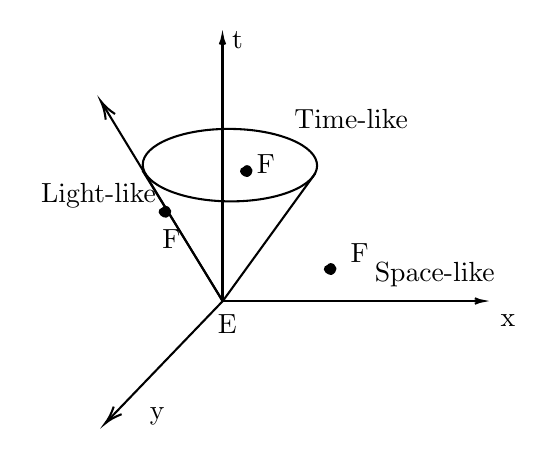
\begin{tikzpicture}[x=0.3pt,y=0.3pt,yscale=-1,xscale=1]
%uncomment if require: \path (0,514); %set diagram left start at 0, and has height of 514

%Straight Lines [id:da2496231248179689] 
\draw    (283.4,350) -- (283.4,32) ;
\draw [shift={(283.4,30)}, rotate = 90] [color={rgb, 255:red, 0; green, 0; blue, 0 }  ][line width=0.75]    (10.93,-3.29) .. controls (6.95,-1.4) and (3.31,-0.3) .. (0,0) .. controls (3.31,0.3) and (6.95,1.4) .. (10.93,3.29)   ;
%Straight Lines [id:da48991715239983225] 
\draw    (283.4,350) -- (596.25,350) ;
\draw [shift={(598.25,350)}, rotate = 180] [color={rgb, 255:red, 0; green, 0; blue, 0 }  ][line width=0.75]    (10.93,-3.29) .. controls (6.95,-1.4) and (3.31,-0.3) .. (0,0) .. controls (3.31,0.3) and (6.95,1.4) .. (10.93,3.29)   ;
%Straight Lines [id:da7876875807666218] 
\draw    (187,192.74) -- (283.77,350) ;
%Straight Lines [id:da37160522507848837] 
\draw    (395,196.5) -- (283.77,350) ;
%Flowchart: Connector [id:dp041231418813562404] 
\draw   (187.36,185.7) .. controls (187.46,161.6) and (234.55,142.34) .. (292.53,142.68) .. controls (350.52,143.03) and (397.45,162.85) .. (397.36,186.95) .. controls (397.26,211.05) and (350.17,230.32) .. (292.18,229.97) .. controls (234.19,229.63) and (187.26,209.81) .. (187.36,185.7) -- cycle ;
%Shape: Free Drawing [id:dp9863864017318156] 
\draw  [line width=3] [line join = round][line cap = round] (413.85,311.5) .. controls (413.85,312.22) and (413.59,309.98) .. (413.85,309.33) .. controls (414.22,308.37) and (417.68,311.22) .. (413.85,313.67) .. controls (412.72,314.39) and (411.72,311.5) .. (410.46,311.5) ;
%Shape: Free Drawing [id:dp6660943461950496] 
\draw  [line width=3] [line join = round][line cap = round] (214.85,242.5) .. controls (214.85,243.22) and (214.59,240.98) .. (214.85,240.33) .. controls (215.22,239.37) and (218.68,242.22) .. (214.85,244.67) .. controls (213.72,245.39) and (212.72,242.5) .. (211.46,242.5) ;
%Shape: Free Drawing [id:dp29359912906223395] 
\draw  [line width=3] [line join = round][line cap = round] (312.85,193.5) .. controls (312.85,194.22) and (312.59,191.98) .. (312.85,191.33) .. controls (313.22,190.37) and (316.68,193.22) .. (312.85,195.67) .. controls (311.72,196.39) and (310.72,193.5) .. (309.46,193.5) ;
%Straight Lines [id:da489078468263464] 
\draw    (283.4,350) -- (138.04,111.21) ;
\draw [shift={(137,109.5)}, rotate = 58.67] [color={rgb, 255:red, 0; green, 0; blue, 0 }  ][line width=0.75]    (21.86,-6.58) .. controls (13.9,-2.79) and (6.61,-0.6) .. (0,0) .. controls (6.61,0.6) and (13.9,2.79) .. (21.86,6.58)   ;
%Straight Lines [id:da1967175868567953] 
\draw    (283.77,350) -- (143.39,496.06) ;
\draw [shift={(142,497.5)}, rotate = 313.87] [color={rgb, 255:red, 0; green, 0; blue, 0 }  ][line width=0.75]    (21.86,-6.58) .. controls (13.9,-2.79) and (6.61,-0.6) .. (0,0) .. controls (6.61,0.6) and (13.9,2.79) .. (21.86,6.58)   ;

% Text Node
\draw (280,22) node [anchor=north west][inner sep=0.75pt]   [align=left] {{ t}};
% Text Node
\draw (603.48,362) node [anchor=north west][inner sep=0.75pt]   [align=left] {{ x}};
% Text Node
\draw (263,363) node [anchor=north west][inner sep=0.75pt]   [align=left] {{ E}};
% Text Node
\draw (423,277) node [anchor=north west][inner sep=0.75pt]   [align=left] {{ F}};
% Text Node
\draw (196,260) node [anchor=north west][inner sep=0.75pt]   [align=left] {{ F}};
% Text Node
\draw (310,170) node [anchor=north west][inner sep=0.75pt]   [align=left] {{ F}};
% Text Node
\draw (355,115) node [anchor=north west][inner sep=0.75pt]   [align=left] {{ Time-like}};
% Text Node
\draw (452,299) node [anchor=north west][inner sep=0.75pt]   [align=left] {{ Space-like}};
% Text Node
\draw (50,205) node [anchor=north west][inner sep=0.75pt]   [align=left] {{ Light-like}};
% Text Node
\draw (181,475) node [anchor=north west][inner sep=0.75pt]   [align=left] {{ y}};
\end{tikzpicture}
\bigskip

If I have two events and computing $\Delta \tau $ gives a positive result, the separation is \textbf{time-like}.
This means that they could be on the WL of a massive particle moving at constant speed.

\paragraph{Physical meaning of $\Delta \tau $}
It's the time elapsed on a clock of the observer moving between E and F at constant speed.

This means that if I compute $\Delta \tau $ on the frame where the observer it is at rest, i get \[
\Delta \tau = \Delta t'
\]

Lets do an example:
\paragraph{Example}
\begin{figure}
\centering
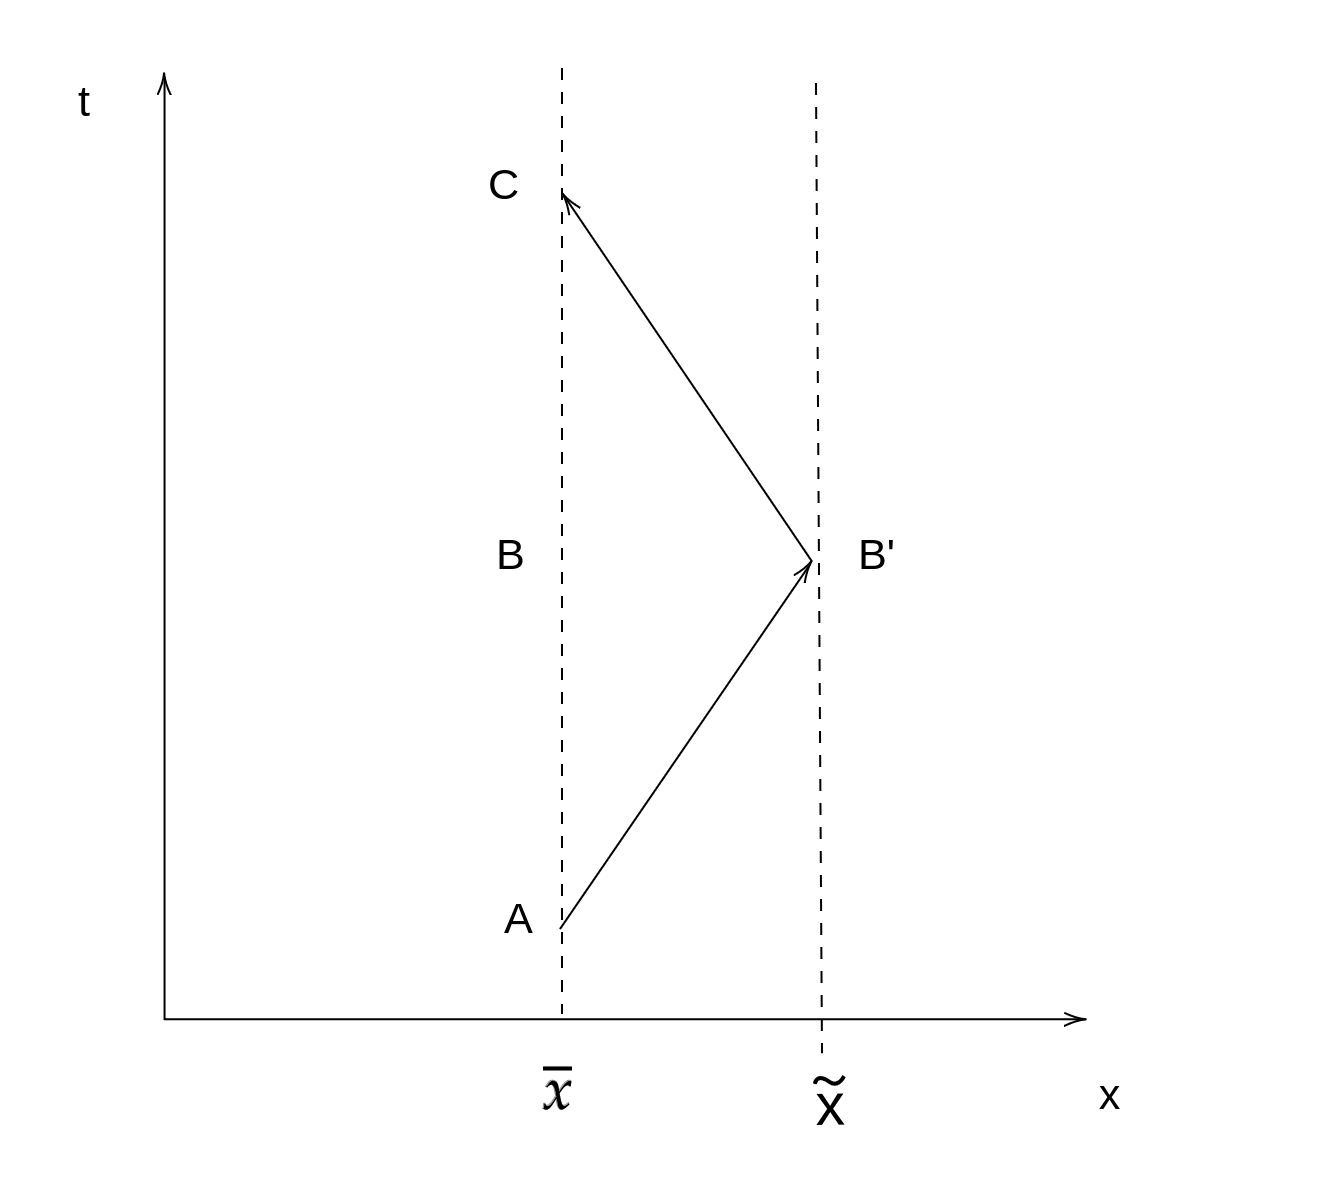
\includegraphics[width=0.6\linewidth]{imm/examplelec3.png}
\caption{It is like the twin paradox.}
\label{imm:examplelec3}
\end{figure}

In fig. \ref{imm:examplelec3} we see the straight line \textbf{ABC} that is the WL of a object not moving. 
Computing its proper time will be:
\begin{equation}
\Delta \tau_{ABC} = \left( t_{c}-t_{A} \right)
\end{equation}
But for the other WL, of a object moving at constant speed between \textbf{AB'} and \textbf{B'C}, we see that

\begin{gather*}
t_{B} = t_{B'} \\
\text{ and so } \\
\Delta \tau_{AB'C} = 2 \sqrt{\left( t_{B} - t_{A} \right)^{2} - \left( \tilde{x} - \bar{x} \right)^{2}} = \Delta \tau_{ABC} \sqrt{1 - \left( \frac{v}{c}  \right)^{2}} \\
\implies \Delta \tau_{AB'C} < \Delta \tau_{ABC}
\end{gather*}

This means that I have the longest \textbf{proper time} when I don't move.

We can do one more generalization: by parametrize the WL with a quantity $\lambda $ we get
\begin{gather*}
x^{\mu }\left( \lambda  \right) \\
\Delta \tau = \int \sqrt{- \eta_{\mu \nu } \frac{dx^{\mu }}{d\lambda } \frac{dx^{\nu }}{d\lambda }} d\lambda \text{ that is a time like trajectory. }
\end{gather*}

Enough with proper time.

\subsection{Tensor Calculus}
Be a Lorentz Group, we want to look for the transformations.
\begin{equation}
x^{\mu } \to x^{\mu'} = \Lambda^{\mu'}_{\mu } x^{\mu }
\end{equation}
we see that it is a linear transformation. An example to see better what are we doing could be
\begin{equation}
x^{0'} = \Lambda^{0'}_{0}x^{0} + \Lambda^{0'}_{1}x^{1} + \Lambda^{0'}_{2}x^{2} + \Lambda^{0'}_{3}x^{3}
\end{equation}
What we need to know is that $\Lambda^{\mu'}_{\mu }$ is a constant matrix.

We see that $\Lambda $   is a constant matrix.

We want to find linear transformations such that 
\begin{equation}
\Delta s^{2} = \eta_{\mu \nu } \Delta x^{\mu }\Delta x^{\nu } = \eta_{\mu' \nu'} \Delta x^{\mu'}\Delta x^{\nu'}
\end{equation}
So the Lorentz Invariant is still invariant. (WTF)

Now, because a SR\footnote{Special Relativity} property: if I move from IF\footnote{Inertial frame} to another, $\eta$ is still unchanged. So \[
\eta_{\mu \nu } = \eta_{\mu' \nu'}
\]

We have to say that Minkowski assumes cartesian coordinates.

The question now is: What trivial transformations leave $\Delta s^{2}$ unchanged?

\paragraph{Translations}
\begin{gather*}
\eta_{\mu  \nu }\Delta x^{\mu }x^{\nu } = \eta_{\mu' \nu'}\left( \Lambda^{\mu'}_{\mu }\Delta x^{\mu } \right) \left( \Lambda^{\nu'}_{\nu }\Delta x^{\nu } \right) \\
\implies \eta_{\mu  \nu } = \eta_{\mu' \nu'} \Lambda^{\mu'}_{\mu }\Lambda^{\nu'}_{\nu } \\
\text{ this obviously needs to be valid } \forall \Delta x^{\mu } \\
\text{ an alternative notation could be } \eta = \Lambda^{T} \eta \Lambda \\
\end{gather*}
We will use just the first notation, because we need to get good at tensors.

To be more concrete:
\begin{equation}
\Lambda^{\mu'}_{\mu } = \begin{pmatrix}
\Lambda^{0'}_{0} & \Lambda^{0'}_{1} & \Lambda^{0'}_{2} & \Lambda^{0'}_{3} \\
\Lambda^{1'}_{0} & ... & ... & ... \\
\Lambda^{2'}_{0} & ... & ... & ... \\
\Lambda^{3'}_{0} & ... & ... & ...
\end{pmatrix} 
\end{equation}

\paragraph{Rotations} 



Rotations are a kind of transformation of the type:
\begin{gather*}
x_{i'} = R_{i i'} x_{i} \\
\text{ or } R^{T} \mathbb{I} R = \mathbb{I} \\
\text{ with } RR^{T} = R^{T}R = \mathbb{I}
\end{gather*}

it could be something like
\begin{equation} \Lambda^{\mu'}_{\mu } = 
\begin{pmatrix}
\text{ cosh } \eta  & - \text{ sinh } \eta   & 0 & 0 \\
- \text{ sinh } \eta  & \text{ cosh } \eta  & 0 & 0 \\
0 & 0 & 1 & 0 \\
0 & 0 & 0 & 1
\end{pmatrix} 
\end{equation}
this one is a boost along the $x$ direction. If we do some computing we find that 
\[
\text{ tanh } \eta \equiv v
\]
so this is the same of the L.T. we saw last week. \par

Rotations do not change the time coordinate. The point was to tell what L.T. is in this language.

\paragraph{Vectors}


I have a generic vector, \textbf{do i need to  specify about the RF} where it is defined, so in a specific spacetime location? {\tiny yes} \par

In newtonian mechanics parallel vectors are the same because I can superpose them, I can move them around, also to use the parallelogram rule to get a sum. \par
$\implies$If I have 3D euclidean space there is no ambiguities about where i move my vectors.\par
\textbf{BUT} in a sphere:

\noindent
\begin{minipage}[t]{0.45\textwidth}
	\vspace*{0pt}
\tikzset{every picture/.style={line width=0.4pt}} %set default line width to 0.75pt        

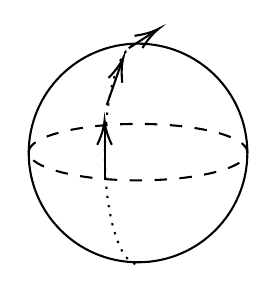
\begin{tikzpicture}[x=0.4pt,y=0.4pt,yscale=-1,xscale=1]
%uncomment if require: \path (0,300); %set diagram left start at 0, and has height of 300

%Shape: Circle [id:dp6654577831806846] 
\draw   (205.5,152.75) .. controls (205.5,98.21) and (249.71,54) .. (304.25,54) .. controls (358.79,54) and (403,98.21) .. (403,152.75) .. controls (403,207.29) and (358.79,251.5) .. (304.25,251.5) .. controls (249.71,251.5) and (205.5,207.29) .. (205.5,152.75) -- cycle ;
%Shape: Ellipse [id:dp25748828027722603] 
\draw  [dash pattern={on 4.5pt off 4.5pt}] (205.5,152) .. controls (205.5,137.92) and (249.71,126.5) .. (304.25,126.5) .. controls (358.79,126.5) and (403,137.92) .. (403,152) .. controls (403,166.08) and (358.79,177.5) .. (304.25,177.5) .. controls (249.71,177.5) and (205.5,166.08) .. (205.5,152) -- cycle ;
%Shape: Arc [id:dp3672101138168469] 
\draw  [draw opacity=0][dash pattern={on 0.84pt off 2.51pt}] (301.86,253.06) .. controls (286.41,249.01) and (274.25,206.07) .. (274.25,153.69) .. controls (274.25,100.16) and (286.95,56.49) .. (302.88,54.1) -- (304.25,153.69) -- cycle ; \draw  [dash pattern={on 0.84pt off 2.51pt}] (301.86,253.06) .. controls (286.41,249.01) and (274.25,206.07) .. (274.25,153.69) .. controls (274.25,100.16) and (286.95,56.49) .. (302.88,54.1) ;  
%Straight Lines [id:da2694092326525188] 
\draw    (274,177.5) -- (274,125.5) ;
\draw [shift={(274,123.5)}, rotate = 90] [color={rgb, 255:red, 0; green, 0; blue, 0 }  ][line width=0.75]    (21.86,-6.58) .. controls (13.9,-2.79) and (6.61,-0.6) .. (0,0) .. controls (6.61,0.6) and (13.9,2.79) .. (21.86,6.58)   ;
%Straight Lines [id:da8503547294122475] 
\draw    (276,109.5) -- (290.34,68.39) ;
\draw [shift={(291,66.5)}, rotate = 109.23] [color={rgb, 255:red, 0; green, 0; blue, 0 }  ][line width=0.75]    (21.86,-6.58) .. controls (13.9,-2.79) and (6.61,-0.6) .. (0,0) .. controls (6.61,0.6) and (13.9,2.79) .. (21.86,6.58)   ;
%Straight Lines [id:da6949662065564377] 
\draw    (295.88,58.1) -- (321.32,41.59) ;
\draw [shift={(323,40.5)}, rotate = 147.02] [color={rgb, 255:red, 0; green, 0; blue, 0 }  ][line width=0.75]    (21.86,-6.58) .. controls (13.9,-2.79) and (6.61,-0.6) .. (0,0) .. controls (6.61,0.6) and (13.9,2.79) .. (21.86,6.58)   ;

\end{tikzpicture}
\end{minipage}
\begin{minipage}[t]{0.48\textwidth}
    \vspace*{0pt} 
    I have this vector at the equator tangent to the surface. If I transport it to the pole i get a different vector.		
\end{minipage}
\bigskip


There are ambiguities. So in a non-flat space we need a \textbf{different} procedure. \par
A vector field is a map between:
\[
x^{\mu } \to v^{\mu }
\]
where $x^{\mu }$ is an event and $v^{\mu }$ is a vector. \par

Let's define: \textbf{Tangent space T\textsubscript{P}}: \par
\noindent Given an event $P$ we define the tangent space $T_{P}$ as all the vectors in $P$.\par

Instead of having spacetime we have a sphere.

\noindent
\begin{minipage}[t]{0.48\textwidth}
    \vspace*{0pt}
    

\tikzset{every picture/.style={line width=0.75pt}} %set default line width to 0.75pt        

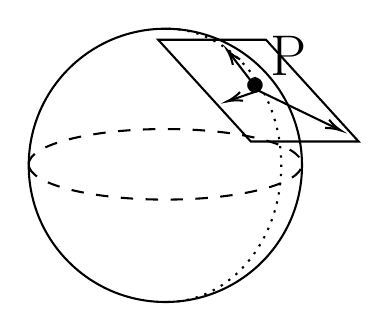
\begin{tikzpicture}[x=0.5pt,y=0.5pt,yscale=-1,xscale=1]
%uncomment if require: \path (0,300); %set diagram left start at 0, and has height of 300

%Shape: Circle [id:dp6654577831806846] 
\draw   (17.5,138.75) .. controls (17.5,84.21) and (61.71,40) .. (116.25,40) .. controls (170.79,40) and (215,84.21) .. (215,138.75) .. controls (215,193.29) and (170.79,237.5) .. (116.25,237.5) .. controls (61.71,237.5) and (17.5,193.29) .. (17.5,138.75) -- cycle ;
%Shape: Ellipse [id:dp25748828027722603] 
\draw  [dash pattern={on 4.5pt off 4.5pt}] (17.5,138) .. controls (17.5,123.92) and (61.71,112.5) .. (116.25,112.5) .. controls (170.79,112.5) and (215,123.92) .. (215,138) .. controls (215,152.08) and (170.79,163.5) .. (116.25,163.5) .. controls (61.71,163.5) and (17.5,152.08) .. (17.5,138) -- cycle ;
%Shape: Arc [id:dp3672101138168469] 
\draw  [draw opacity=0][dash pattern={on 0.84pt off 2.51pt}] (118.33,237.5) .. controls (163.51,236.96) and (200,192.96) .. (200,138.75) .. controls (200,84.76) and (163.8,40.88) .. (118.86,40.01) -- (117.5,138.75) -- cycle ; \draw  [dash pattern={on 0.84pt off 2.51pt}] (118.33,237.5) .. controls (163.51,236.96) and (200,192.96) .. (200,138.75) .. controls (200,84.76) and (163.8,40.88) .. (118.86,40.01) ;  
%Shape: Parallelogram [id:dp887464464445318] 
\draw   (111.1,48) -- (189,48) -- (255.9,121.5) -- (178,121.5) -- cycle ;
%Straight Lines [id:da3128101776711285] 
\draw    (183.5,84.75) -- (241.2,112.63) ;
\draw [shift={(243,113.5)}, rotate = 205.79] [color={rgb, 255:red, 0; green, 0; blue, 0 }  ][line width=0.75]    (10.93,-3.29) .. controls (6.95,-1.4) and (3.31,-0.3) .. (0,0) .. controls (3.31,0.3) and (6.95,1.4) .. (10.93,3.29)   ;
%Straight Lines [id:da05720579900710121] 
\draw    (183.5,84.75) -- (162.22,57.09) ;
\draw [shift={(161,55.5)}, rotate = 52.43] [color={rgb, 255:red, 0; green, 0; blue, 0 }  ][line width=0.75]    (10.93,-3.29) .. controls (6.95,-1.4) and (3.31,-0.3) .. (0,0) .. controls (3.31,0.3) and (6.95,1.4) .. (10.93,3.29)   ;
%Straight Lines [id:da5083189086137138] 
\draw    (183.5,84.75) -- (162.89,91.85) ;
\draw [shift={(161,92.5)}, rotate = 340.99] [color={rgb, 255:red, 0; green, 0; blue, 0 }  ][line width=0.75]    (10.93,-3.29) .. controls (6.95,-1.4) and (3.31,-0.3) .. (0,0) .. controls (3.31,0.3) and (6.95,1.4) .. (10.93,3.29)   ;

% Text Node
\draw (172,73.4) node [anchor=north west][inner sep=0.75pt]  [font=\Large]  {$\bullet $};
% Text Node
\draw (190,43) node [anchor=north west][inner sep=0.75pt]   [align=left] {{\huge P}};


\end{tikzpicture}

\end{minipage}
\begin{minipage}[t]{0.48\textwidth}
    \vspace*{0pt} 
	Define a plane tangent to the sphere only in $P$. All vectors that lie there $\in T_{P}$.    
\end{minipage}
\bigskip


$T_{P}$ is a \textbf{vector space}:
\[
	V,W \in T_{P} \implies \alpha V + \beta W, \left( \alpha , \beta \in \mathbb{R} \right) \in T_{P}
\]
So if there is a vector there is also the inverse vector.\par
Whenever I have a vector space, I can define infinite basis independently on the coordinate choice. The number of elements in the basis is equal to the dimension of the space, in our case 4 elements.\par
Obviously if I define the basis its elements need to be Linearly Independent. 

\paragraph{Basis}
Given a generic vector $V \in T_{P}$, I can define $V$ regardless the coordinate system I'm using. So we can say \emph{metaphorically} that $V$ exists before I define coordinates.\par
Be our basis:
\[
\hat{e}_{\left( \mu  \right)}, \text{ with } \mu = 0,1,2,3	
\]
those indices are label, does not mean "tensor". So my basis is made of \[
\hat{e}_{\left( 0 \right)}, \hat{e}_{\left( 1 \right)}, \hat{e}_{\left( 2 \right)}, \hat{e}_{\left( 3 \right)}
\]
Now we can talk about
\paragraph{Components}
given a generic vector $V$ 
\[
V = V^{0}\hat{e}_{\left( 0 \right)} + V^{1}\hat{e}_{\left( 1 \right)} + V^{2}\hat{e}_{\left( 2 \right)} + V^{3}\hat{e}_{\left( 3 \right)} =  V^{\mu }\hat{e}_{\left( \mu  \right) }
\]
using repeating indices we get the last equivalence.

$V^{\mu }$ are components of the vector $V$ in this specific frame. \par
In another frame $V^{\mu '}$ could not be the same:
\[
	V = V^{\mu }\hat{e}_{\left( \mu  \right)} = V^{\mu '}\hat{e}_{\left( \mu ' \right)}
\]

\textbf{Question:} how do components transform?
\paragraph{Contravariant vector}: is a math object whose components transform based on position
\[
V^{\mu '} = \Lambda^{\mu '}_{\mu }V^{\mu }
\]
These are not the only covariant vectors (?).

If you have a generic WL or path, you can parametrize the position by a $\lambda$ in this way:
\[
x^{\mu }\left( \lambda  \right)
\]
And taking its first derivative you get something similar to the four-velocity
\[
u^{\mu }\sim \frac{dx^{\mu }}{d\lambda }
\]
(I say similar because four-velocity is defined like $u^{\mu } = \frac{dx^{\mu }}{d\tau }$).

If I do a L.T. $x^{\mu }$ will change but $\lambda $ won't.
\[
u^{\mu '} = \Lambda^{\mu '}_{\mu }u^{\mu }
\]
I can get a more general definition of what a vector is by following this procedure:
choose basis $\to$ find components $\to$ study how components change if i change position or basis.

\paragraph{Second definition}: Transformation of the basis vectors. The question is "how to relate $\hat{e}_{\left( \mu  \right)}$ to $\hat{e}_{\left( \mu ' \right)}$?"

We will take advantage of \textbf{invariance}. 
\[
V = V^{\mu }\hat{e}_{\left( \mu  \right) } = V^{\mu '}\hat{e}_{\left( \mu ' \right)} = \left( \Lambda^{\mu '}_{\mu }V^{\mu } \right)\hat{e}_{\left( \mu ' \right)}
\]
That's possible \textbf{only} if $\hat{e}_{\left( \mu  \right)} = \Lambda^{\mu '}_{\mu }\hat{e}_{\left( \mu ' \right)}$.

An inverse of LT it is also a LT, so
\begin{gather*}
\Lambda^{\mu '}_{\mu }\Lambda^{\mu }_{\nu '} = \delta^{\mu '}_{\nu '} \\
\Lambda^{\mu }_{\mu '}\Lambda^{\mu '}_{\nu } = \delta^{\mu }_{\nu }	
\end{gather*}
Those are Kroneker's delta and they are an Identity matrix.

Now we can study how basis vectors change.
\begin{gather*}
\hat{e}_{\left( \mu  \right)} = \Lambda^{\mu '}_{\mu }\hat{e}_{\left( \mu ' \right)} \\
\Lambda^{\mu }_{\nu '}\hat{e}_{\left( \mu  \right)} = \Lambda^{\mu '}_{\mu }\Lambda^{\mu }_{\nu '} \hat{e}_{\mu '} \\
\Lambda^{\mu }_{\nu '}\hat{e}_{\left( \mu  \right)} = \delta^{\mu '}_{\nu '}\hat{e}_{\left( \mu ' \right)} \\
\Lambda^{\mu }_{\nu '}\hat{e}_{\left( \mu  \right)} = \hat{e}_{\left( \nu ' \right)} \\ 
\text{ so } \hat{e}_{\left( \nu ' \right)} = \Lambda^{\mu }_{\nu '}\hat{e}_{\left( \mu  \right)}
\end{gather*}
